\chapter[Results]{Results}
\label{sec:results}

This chapter explains the results obtained with the project development. Section \ref{sec:template} gives an explanation of how the model works, how it is divided and what files come when downloading it. It also explains what each file is responsible for and if the user should edit it or not. Section \ref{sec:difficulties} shows some of the problems that came through the development/maintenance of the template and how they were overcome.


\section{Template}
\label{sec:template}

One of the goals of this work was to generate a template that allowed the game developers from the courses of this University to create their games and quickly create packages to install in major Operating Systems, namely, Windows, macOS, Debian-based and Red Hat based distributions of GNU/Linux. Professor Edson made this template.  I had the responsibility of testing it in a few games, evolving and maintaining it throughout all the platforms.

The template consists of a series of Bash scripts, Makefile, libraries and a directory structure that is supposed to be followed by anyone who wants to use it. It is intended to be used as a template for new games developed in the courses taught at this University, and it contains the most common libraries in game development, like SDL, SDL\_image, and SDL\_mixer.

\subsection{Root directory}
\label{sec:root_directory}

Currently, there are seven required files on the root directory, specifically, \texttt{LICENSE}, \texttt{Makefile.common}, \texttt{Makefile.macos}, \texttt{Makefile.windows}, \texttt{Makefile.linux}, \texttt{Vagranfile}, \texttt{changelog}, and \texttt{metadata.ini}. These files assure compilation is possible in any platform and also give some information about the project. An explanation of what each of them does and what information each may or may not have is given on Table \ref{tab:files_root_dir}. Some extra optional files are also explained.


\begin{longtabu} to \linewidth {XlX[2]}

\caption{Files on the root directory}\label{tab:files_root_dir}\\
\toprule
\textbf{File} & \textbf{Mode} & \textbf{Description} \\
\midrule
\endhead

% \\ \hline
% \multicolumn{3}{r}{There is more to come} \\
% \endfoot

% \\ \hline
% \endlastfoot

\texttt{LICENSE} & \emph{Editable.} & This should be the text of the license or a reference to a file that has the full text. Debian packages complain if this file is the actual license text for common licenses, therefore it may be better option to only refer to a file inside the system (usually \texttt{/usr/share/common-licenses/<LICENSE>}); \\ \hline
\texttt{Makefile.macos} \texttt{Makefile.windows} \texttt{Makefile.linux} & \emph{Uneditable.} & Each of these files sets variables with specific for each system, like \texttt{CC} and \texttt{DEBUG\_FLAGS}. If a variable isn't needed it will remain blank and won't change the effect of the compilation. The template is supposed to work with values as they are and users shouldn't change them unless they \emph{actually} want a different behavior. \\ \hline
\texttt{Makefile.common} & \emph{Partially editable.} & Sets some other variables, common to all OSs, like \texttt{LDFLAGS}, based on each platform Makefile. The template has set default SDL libs (SDL, SDL\_image, SDL\_mixer, SDL\_ttf), but other external libs may be wanted. When this happens, the user should add the libs wanted to the variable \texttt{EXTERNAL\_LIBS} without quotes and separated by simple space. Each of these libs must be a directory inside the \texttt{lib} folder. The rest of the file should not be changed since it may lead to major errors when using the template unless the user is sure of how it works. \\ \hline
\texttt{Vagranfile} & \emph{Optional.} & This file creates two Virtual Machines running Debian and CentOS. If the user wishes to give support for them both (generating both \texttt{.deb} and \texttt{.rpm} packages), they could either use the VMs or run the template natively on each system. The virtualization provides an easier way to do that, but it is up to the user deciding this detail of the development cycle. \\ \hline
\texttt{changelog} & \emph{Editable.} & When creating the Debian package, it needs a changelog, that registers what was changed from the previous versions, much like a commit message. There are ways of generating this file automatically because its syntax is very particular, but the template doesn't contemplate it yet. \\ \hline
\texttt{metadata.ini} & \emph{Editable.} & As the extension suggests, \textit{ini} stands for \textit{initialization}. It is a configuration file that follows the \texttt{ini} syntax. It defines some project properties that will be used in several steps, like building and packaging, making it a critical file to use the template correctly. The user should change this file with the appropriate information as soon as cloning the repository and throughout the development. \\

\bottomrule
\end{longtabu}


\subsection{Sources Directory (\texttt{src})}
\label{sec:src_folder}

The directory that holds all source code, including headers, is called \texttt{src} and is divided in two subfolders, \texttt{engine} and \texttt{game}, as shown in Figure \ref{fig:folder_structure_src}. The reason for this division is to keep separate what is engine specific (like movements, rendering windows, capturing input from the player) from the actual game. Engines can be reused in several projects, providing a basic API to create new games. Both of these directories have the same structure, that is explained in Table \ref{tab:files_src_dir}, along with the files outside them.

\begin{longtabu} to \linewidth {XlX[2]}

\caption{Files in the sources directory}\label{tab:files_src_dir}\\
\toprule
\textbf{File} & \textbf{Mode} & \textbf{Description} \\
\midrule
\endhead

\texttt{main.cpp} & \textit{Partially Editable.} & It is where the function \texttt{main} should live. This file must not be renamed or moved to inside any of the subdirectories. Users should add their logic to it, with all the relative includes. Because of compatibility issues with Windows, there is a function called \texttt{WinMain}, that only calls the main function and should not be touched. \\ \hline
\texttt{Makefile} & \textit{Uneditable.} & This makefile is called during the build process, from inside \texttt{Makefile.common}. It builds the final executable, linking main with the game library, engine library, and the libraries inside \texttt{lib}. \\ \hline
\texttt{\{game,engine\}/ include/*} & \textit{Editable.} & These are the header files for the engine and the game. The template already has one header in the engine, that should not be removed, but may be renamed if the correct references are made after that. This header defines the function \texttt{resources\_dir\_path}, that is very important to keep the template ability to run on multiple platforms. \\ \hline
\texttt{\{game,engine\}/ src} & \textit{Editable.} & The implementation of all header functions should go inside this directory. Under this three other directories are supposed to hold platform-specific implementation, namely, \texttt{linux, windows,} and \texttt{macos}. Any code outside them is considered to be generic and can be used in any of these platforms. Every piece of code specific to one of these systems should be placed in the corresponding folder. The template already has the specific implementation to find the \texttt{resources} folder that may be renamed or reimplemented. It is not advised to change the \texttt{macos} implementation though, except for the directory name. \\ \hline
\texttt{\{game,engine\}/ Makefile} & \textit{Uneditable.} & Called from the \texttt{Makefile} in the \texttt{src} directory. Responsible for building each of these two libraries. If the folder structure was followed correctly, there is no need to change the contents of this file. \\

\bottomrule
\end{longtabu}



\begin{figure}[h!]
\centering
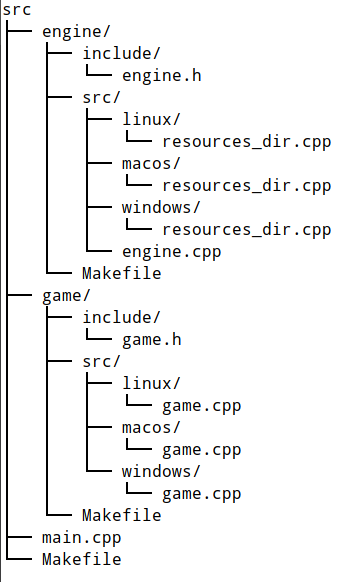
\includegraphics[height=300px,keepaspectratio]{folder_structure_src}
\caption{\texttt{src} directory}
\label {fig:folder_structure_src}
\end{figure}

\subsection{Distribution folder (\texttt{dist})}
\label{sec:dist_folder}

Each platform has particularities concerning generating packages. Debian, for example, requires a changelog inside the package, while Windows needs to have the package registered (with all of its contents). The dist folder contains some specific files that are needed for each package. Figure \ref{fig:folder_structure_dist} shows the files needed for each system, while Table \ref{tab:files_dist_dir} explains what is of them is supposed to do.

\begin{figure}[h!]
\centering
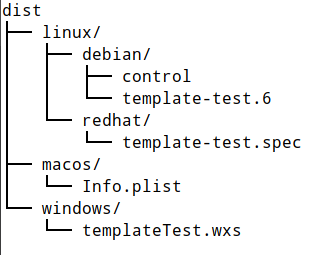
\includegraphics[height=200px, keepaspectratio]{folder_structure_dist}
\caption{\texttt{dist} directory}
\label {fig:folder_structure_dist}
\end{figure}

\begin{longtabu} to \linewidth {XlX}

\caption{Files on the \texttt{dist} directory}\label{tab:files_dist_dir}\\
\toprule
\textbf{File} & \textbf{Mode} & \textbf{Description} \\
\midrule
\endhead

\texttt{windows/templateTest.wxs} & \textit{Uneditable.} & This file is required to generate the installer for windows. It is an XML that lists all directories, files and libraries inside the installer. Each one of them has a unique UUID, because this is how Windows controls what is installed or removed. This file is generated once when \texttt{pack.sh} called in Windows. If the user has updated the resources and other files, they should delete this and rerun \texttt{pack.sh}, but never edit it themselves, because it is a very particular \textbf{large} file. \\ \hline
\texttt{macos/Info.plist} & \textit{Uneditable.} & Because macOS packages are self-contained, this file is pretty simple. It is an XML that contains keys and values related to the package installed, like its name, version, and developer. This file has its information updated when \texttt{pack.sh} is called on a macOS system. \\ \hline
\texttt{linux/redhat/template-test.spec} & \textit{Uneditable.} & Every \texttt{rpm} package has to have a file containing the isntructions of what to and how to install that package. This file is replaced with the specifics of each game, mostly the information in \texttt{metadata.ini}, when \texttt{pack.sh} is called on a Red Hat machine. \\ \hline
\texttt{linux/debian/control} & \textit{Uneditable.} & Inside a debian package, there is a control section, that contains some metadata for the package being installed. It is a required file on every \texttt{.deb} package. This file has this data, aquired from \texttt{metadata.ini}. \\ \hline
\texttt{linux/debian/template-test.6} & \textit{Uneditable.} & Even though this file is inside \texttt{debian}, it is used for both linux distributions. It is a \texttt{man} file, that contains the package usage description. \\
\bottomrule
\end{longtabu}




\subsection{Scripts folder (\texttt{scripts})}
\label{sec:scripts_folder}

A central part of the template is the ability to build, run and package the game. This ability happens because several scripts allow users to quickly do this process, by running them from the root directory of the repository. None of these files should be modified by the user.

The scripts inside this folder are not complex or complicated since the hard work is mostly done inside the \texttt{util} directory. The build script is fairly simple, requiring one argument that is the mode the script will run, \texttt{debug} or \texttt{release}. If none is provided, it will use \texttt{debug} as default. It simply checks the platform and run the command \texttt{make} with the appropriate Makefile and mode; \texttt{run.sh} sets some variables and change the directory to where all the libs are to then call the executable; \texttt{cleanup.sh} remove objects, libraries and other files generated during compilation; and \texttt{pack.sh} calls one of the scripts inside \texttt{util} to generate the corresponding package.

Generating a \texttt{.deb} package consists in a few steps as shown in Listing \ref{lst:gen_deb.sh}. It first sets some variables and loads info from \texttt{metadata.ini}, in lines 7-11. When the function \texttt{gen\_deb()} is called, it creates a temporary directory and its structure, in lines 9 through 24. From line 26 through 43, the executable, the required libs, and the resources are all copied to their respective location inside this structure. The \texttt{control} file is copied from \texttt{dist} folder and the information is replaced with what is in \texttt{metadata.ini} in lines 46-59. Lines 62-75 create some other directories, copy license, changelog and man pages to a documentation folder, and compress some of the files. Lines 77-88 set the correct permissions, strip the executable, builds and checks the package for errors.

\lstinputlisting[language=bash, frame=single, caption={\texttt{gen\_deb.sh}}, label=lst:gen_deb.sh]{../proj-template/scripts/util/gen_deb.sh}

Making an \texttt{.rpm} package is somewhat simpler than generating a Debian package. As seen in Listing \ref{lst:gen_rpm.sh}, \texttt{gen\_rpm.sh} starts on lines 7-11 also loading \texttt{metadata.ini} and defining some variables. When \texttt{gen\_rpm()} is called, it first calls the rpm tool that creates a folder structure for the package, on line 18. After that, on lines 21 - 29, it copies the spec file to its place on that structure and replaces the information read from \texttt{metadata.ini}. Line 32 puts the text script that will be executed in the folder structure. Lines 35-39 remove any traces of other times this script was called and create a \texttt{tar} package based on the structure the rpm builder created. Lines 42-44 build the \texttt{rpm} package and calls the lint to check it. Unlike Debian, everything the builder needs to know is inside the \texttt{spec} file; the script only copies things to where they are supposed to be.

\lstinputlisting[language=bash, frame=single, caption={\texttt{gen\_rpm.sh}}, label=lst:gen_rpm.sh]{../proj-template/scripts/util/gen_rpm.sh}

To generate the Windows installer, the script \texttt{gen\_exe.sh} is called. It starts, in lines 7-11, loading and setting variables just like the other scripts. When \texttt{gen\_exe()} is called, it makes the folder where all the libs and resources will live, in lines 14-15. Lines 17-20 copy the release libs to the folder created in the previous step. Lines 22-25 create a new \texttt{wxs} file, only if one doesn't exist. This decision was made because it takes a lot of time to create that file. If the user wants to recreate it, they just have to delete it from the \texttt{dist} folder. Lines 27-36, copy all the libs, resources, executable and wxs to a temporary directory. Lines 38-41 do the actual package building, calling \texttt{candle.exe} and \texttt{light.exe} that are Wix tools that compile the \texttt{.wxs} file into \texttt{.wxsobj} and create the \texttt{.msi}, respectively.

\lstinputlisting[language=bash, frame=single, caption={\texttt{gen\_exe.sh}}, label=lst:gen_exe.sh]{../proj-template/scripts/util/gen_exe.sh}


\section{Difficulties}
\label{sec:difficulties}

Creating the installer for Windows has proved to be the hardest part of the template because Windows has an entirely different folder structure from GNU/Linux systems, they also don't have the same tools available (like Bash). Compiling for Windows has also turned out to be more challenging than Professor Edson first anticipated, because the template wouldn't run correctly, even after installing all required dependencies.

The template for Windows was supposed to use Visual Studio compiler, which is a tool made specifically for that platform, however when calling the compiler, it would not find any of the \texttt{.cpp} files. To try to revert that situation, the parameters passed to the compiler inside \texttt{Makefiles} were checked and the compiling commands were run individually inside each folder that had the source code. Even after that thorough examination, the compiler would refuse to find the files. All tools were uninstalled and reinstalled, and the problem remained. It was decided to change the compiler to \texttt{gcc} to solve this issue, just like the GNU/Linux systems.

Changing the compiler was partially natural because it was needed only to replicate the Linux \texttt{Makefile} on Windows (with a few commands replaced). It was required to install one more dependency, the compiler, and its stack, but Visual Studio could be dropped too. This error has caused another complication, because, for some reason, during the final part of the compilation, it didn't recognize the \texttt{main} function. It turns out that the compiler needed a different entry point instead of the default \texttt{main}. According to Visual Studio documentation, when creating a GUI application, it requires a function called \texttt{WinMain} \cite{visualstudio2017entrypoint} and even with \texttt{mingw} it complained about not having it. This function was added, and it simply called \texttt{main}.

After compiling, the issue was to generate the installer. Initially, the script didn't provide any means to create the required \texttt{wxs} with the data from the repository, demanding the user to create that file manually. It wasn't an easy task, since this is a very particular large file, with specific tags, keywords, and syntax. For example, every independent set of data must be wrapped around a component, (that is how Windows checks what is what inside a package) and each of the resources inside the package must be listed).

To aid in that process, the script \texttt{gen\_wxs} was created and the \texttt{wxs} generation was divided into three parts, header, directory, and feature, just to make it easier to generate the whole file. The main problem in this part of the template development was finding and listing the resources because there could be any number of subdirectories. Recursion was the first idea to solve this issue, as seen lines 189-207 of Listing \ref{lst:gen_wxs.sh}, but it proved to be hard to use in Bash because it defines variables only once. The recursive variable had to be updated, to solve that issue, before returning to the previous call. The command in line 206 of Listing \ref{lst:gen_wxs.sh} removes everything in the name of the file until the last \texttt{/}, assuring that \texttt{\$FILE\_PATH} has the correct value on the next recursive call. By doing that, it was possible to list all resources and their folders in the \texttt{wxs} file.

\lstinputlisting[language=bash, frame=single, caption={Part of \texttt{gen\_wxs.sh}}, label=lst:gen_wxs.sh, firstnumber=189, firstline=189, lastline=207]{../proj-template/scripts/util/gen_wxs.sh}


Another challenge in testing the template was the migration to SDL2. Even though it was intended to be used with SDL2 since the beginning, Professor Edson chose to start with SDL and then add support to the newer version. The games initially selected for this part were \textit{Traveling Will} and \textit{Deadly Wish}, from the beginning of 2015. Even though they work fine when the libs are installed, there was a problem using them to test the template, because they needed the external engine created for the course a few years ago. This engine was built to be used as a shared library, which is fine and encouraged, but it expected a different folder structure then the template offered. Even after a few minor changes in it, the game still didn't adequately run when packaged. These errors might be happening from the version of the engine being used because the games didn't specify which they needed. Since the goal of this work was to test the template and not to fix/maintain the engine or the games, \textit{Traveling} and \textit{Deadly} were dropped. The new games selected were \textit{Wenova} and \textit{Mindscape}, both developed on the first semester of 2017.

Changing the template to support SDL2 was a little tricky. Different than the previous SDL version, on Linux the libraries didn't work on both of the desired distributions out of the box, requiring specific binaries for Debian based systems and Red-Hat based systems. Still on Linux, playing \texttt{.mp3} files proved to be slightly more complicated in SDL2. To read that extension SDL\_mixer needs to be compiled with the \texttt{smpeg} library, that will be loaded as a shared lib with the program. Even with the library installed, SDL\_mixer would refuse to open \texttt{.mp3} songs, saying it wasn't a recognized format. The solution came after carefully observing the output of the \texttt{configure} script, that checks which dependencies and third party libs are installed in the computer building SDL. It turns out that SDL2\_mixer required version 2 of \texttt{smpeg}, but that wasn't discriminated anywhere in their documentation. SDL\_mixer 1, used version 0.4.5 of \texttt{smpeg}, the one that comes in the distro repositories, and worked fine because of that.

On Windows, the problem was loading the images of \textit{Wenova}. Since \texttt{mingw} is being used as compiler for Windows, the \texttt{mingw} binaries were downloaded. It turns out that, for some reason, SDL\_image would not load \texttt{.png} files, due to \texttt{libpng} having some reference to some function that wasn't defined in any part of it or its dependencies. The error on the console wasn't of any help, and the internet searches would only result in adding \texttt{zlib1} to the dependencies, which was already done. In an attempt to correct the error, just to try something, I unzipped the Visual Studio binaries, which in theory wouldn't run on \texttt{mingw} and tried recompiling the game. For some unknown reason, probably all the dependencies were corectly put inside this version of \texttt{libpng}, the game ran correctly this time.

\textit{Mindscape} was probably the hardest game to compile in both platforms, because of a silly mistake the developers made, that was masked in the source code. For some reason, maybe incorrectly merging developing branches or change of the initial plans for the game, they had defined two headers called \texttt{game.hpp}, one in the engine, the other in the game. When creating a C/C++ header, it's a good practice to guard it against multiple imports using a \texttt{\#IF\_N\_DEF} macro that will prevent users to import the same header accidentally (redefining it) \cite{disch_2009}. The team that made \texttt{Mindscape} naturally used this guarding against multiple imports, but they hard referenced all of their imports, therefore always importing the engine \texttt{game.hpp}, that had all the definitions they needed. The template works differently, passing the path of the headers to the compiler, instead of putting that address hardcoded in the source code. Because of that, when removing the full path in the \texttt{.cpp} files, the compiler would find the first defined \texttt{game.hpp}, which was in the game folder. This file had no definitions other the constructor and the destructor, causing a lot of \texttt{Undefined reference} errors during compilation. It took a long time to find out, and it was almost an accident, that there were two of these files, one empty and the other with all the functions correctly defined. Once this was solved, the game compiled and ran successfully.

% Even with all these dificulties a lot of problems

% One more problem with \textit{Mindscape} is the Windows executable, that seems to be missing something, because it won't run
